\documentclass[a4paper,12pt]{scrartcl}
\usepackage{framed}
\usepackage{enumitem}
\usepackage{todonotes}

\usepackage[utf8]{inputenc}
\usepackage{amsfonts}
\usepackage{listings}
\usepackage{hyperref}
\usepackage{listings}
\usepackage{color}
\definecolor{verylightgray}{RGB}{244,244,244}
\definecolor{lightgray}{RGB}{232,232,232}
\definecolor{listinggray}{gray}{0.9}
\definecolor{lbcolor}{rgb}{0.9,0.9,0.9}
\definecolor{gray}{rgb}{0.4,0.4,0.4}
\definecolor{darkblue}{rgb}{0.0,0.0,0.6}
\definecolor{cyan}{rgb}{0.0,0.6,0.6}
\definecolor{dkblue}{rgb}{0,0.1,0.5}
\definecolor{dkgreen}{rgb}{0,0.4,0}
\newcommand{\code}[1]{\colorbox{listinggray}{\texttt{#1}}}
\lstset
{
  captionpos=b,
  basicstyle=\small\ttfamily,
  columns=fullflexible,
  showstringspaces=false,
  commentstyle=\color{gray}\upshape,
  numbers=left,
  stepnumber=1,
  tabsize=2,
  keepspaces=true,
  frame=lines,
  keywordstyle=\color{blue},
  framesep=2pt,
  prebreak=\raisebox{0ex}[0ex][0ex]{\ensuremath{\hookleftarrow}},
  breakindent=4em,
  breaklines=true
}
\lstdefinelanguage{CPP}
{
 morecomment = [l][\color{dkgreen}]{//}, 
 morecomment = [l][\color{dkgreen}]{///},
 morecomment = [s][\color{dkgreen}]{/*}{*/},
 morestring=[b]", 
 sensitive = true,
 morekeywords = {abstract,  event,  new,  struct,
   as,  explicit,  null,  switch,
   base,  extern,  object,  this,
   bool,  false,  operator,  throw,
   break,  finally,  out,  true,
   byte,  fixed,  override,  try,
   case,  float,  params,  typeof,
   catch,  for,  private,  uint,
   char,  foreach,  protected,  ulong,
   checked,  goto,  public,  unchecked,
   class,  if,  readonly,  unsafe,
   const,  implicit,  ref,  ushort,
   continue,  in,  return,  using,
   decimal,  int,  sbyte,  virtual,
   default,  interface,  sealed,  volatile,
   delegate,  internal,  short,  void,
   do,  is,  sizeof,  while,
   double,  lock,  stackalloc,   
   else,  long,  static,   
   enum,  namespace,  string, template, typename, include, nullptr, chan, clock},
 emph={},
 emphstyle=\color{blue},
 emph={[2]value},
 emphstyle={[2]\textbf}
}

\title{Verification mini-project}
\subtitle{Crossing the River}
\author{Jacob Karsten Wortmann\\Sam Sepstrup Olesen\\Nicklas Andersen\\\textit{sw805f14}}

\begin{document}
\maketitle %project description

\begin{itemize}
\item Max 2 persons on the boat,
\item Mom not alone with boys,
\item Dad not alone with girls,
\item Thief not alone with family,
\item Only police officer, dad and mom can handle the boat.
\end{itemize}

\begin{figure}[h]
\centering
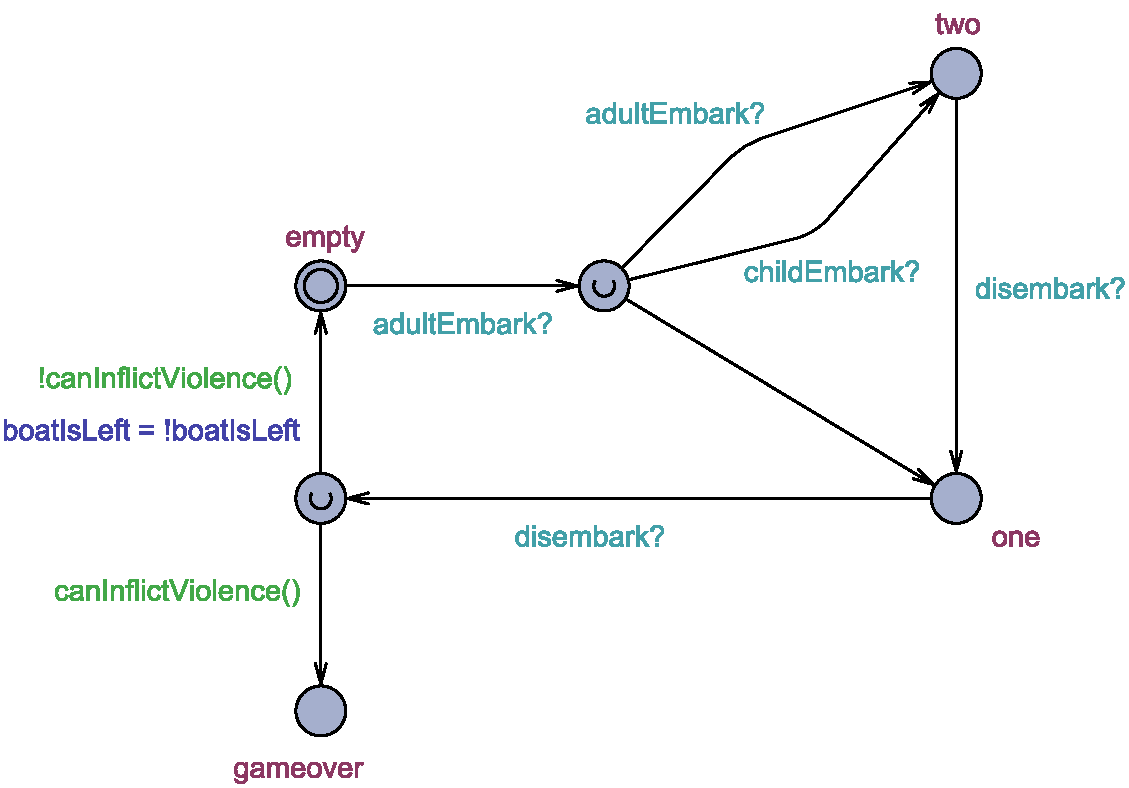
\includegraphics[width=\linewidth]{Boat.pdf}
\caption{Boat.}
\label{fig:boat}
\end{figure}

\begin{figure}[h]
\centering
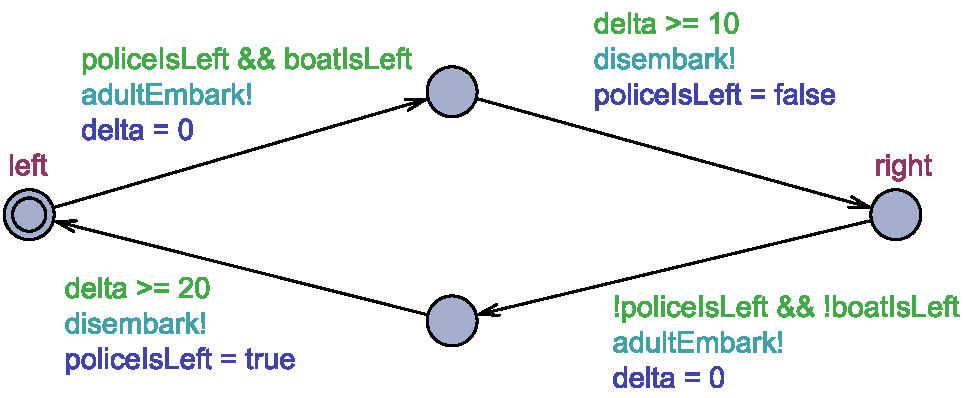
\includegraphics[width=0.7\linewidth]{Police.pdf}
\caption{Police.}
\label{fig:police}
\end{figure}

\begin{figure}[h]
\centering
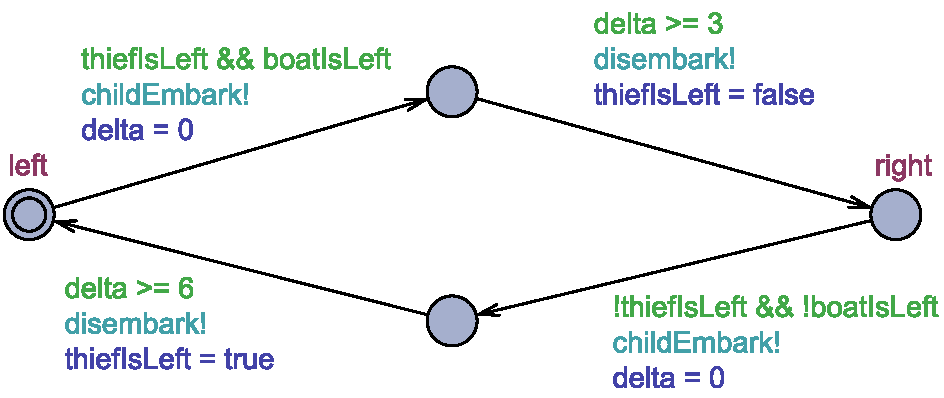
\includegraphics[width=0.7\linewidth]{Thief.pdf}
\caption{Thief.}
\label{fig:thief}
\end{figure}

\begin{lstlisting}[language=CPP, label = lst:plugin_example, caption = Global declaration.]
clock time;

chan adultEmbark, childEmbark, disembark;

bool boatIsLeft = true;

bool policeIsLeft = true;
bool thiefIsLeft  = true;
bool dadIsLeft    = true;
bool momIsLeft    = true;
bool boy1IsLeft   = true;
bool boy2IsLeft   = true;
bool girl1IsLeft  = true;
bool girl2IsLeft  = true;


bool canInflictViolence() {
    if (((momIsLeft == boy1IsLeft)
    	|| (momIsLeft == boy2IsLeft))
    	&& (momIsLeft != dadIsLeft))
        return true;

    if (((dadIsLeft == girl1IsLeft)
    	|| (dadIsLeft == girl2IsLeft))
    	&& (dadIsLeft != momIsLeft))
        return true;

    if (((thiefIsLeft == boy1IsLeft)
    	|| (thiefIsLeft == boy2IsLeft)
    	|| (thiefIsLeft == girl1IsLeft)
    	|| (thiefIsLeft == girl2IsLeft)
    	|| (thiefIsLeft == dadIsLeft)
    	|| (thiefIsLeft == momIsLeft))
    	&& (thiefIsLeft != policeIsLeft))
        return true;

    return false;
}
\end{lstlisting}

\begin{figure}[h]
\centering
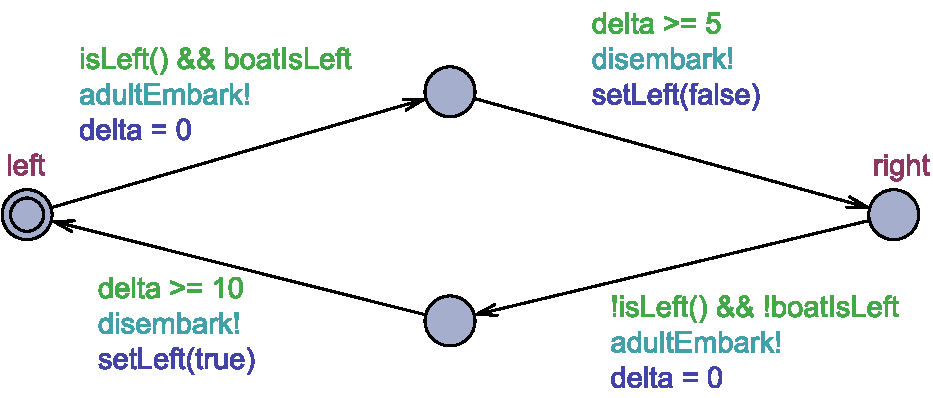
\includegraphics[width=0.7\linewidth]{Parent.pdf}
\caption{Parent.}
\label{fig:parent}
\end{figure}

\begin{lstlisting}[language=CPP, label = lst:plugin_example, caption = Parent declaration.]
clock delta;

bool isLeft() {
    if (isDad)
        return dadIsLeft;
    else
        return momIsLeft;
}

void setLeft(bool left) {
    if (isDad)
        dadIsLeft = left;
    else
        momIsLeft = left;
}
\end{lstlisting}

\begin{lstlisting}[language=CPP, label = lst:plugin_example, caption = Child declaration.]
clock delta;

bool isLeft() {
    if (isBoy)
        if (isFirst)
            return boy1IsLeft;
        else
            return boy2IsLeft;
    else
        if (isFirst)
            return girl1IsLeft;
        else
            return girl2IsLeft;
}

void setLeft(bool left) {
    if (isBoy)
        if (isFirst)
            boy1IsLeft = left;
        else
            boy2IsLeft = left;
    else
        if (isFirst)
            girl1IsLeft = left;
        else
            girl2IsLeft = left;
}
\end{lstlisting}

\begin{figure}[h]
\centering
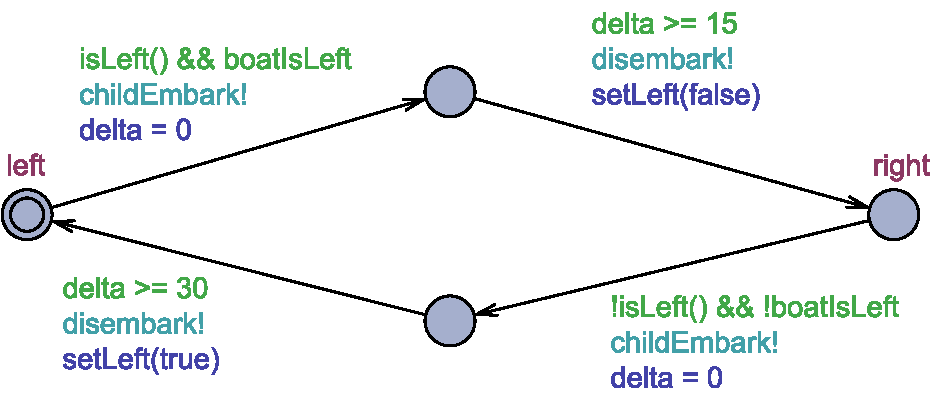
\includegraphics[width=0.7\linewidth]{Child.pdf}
\caption{Child.}
\label{fig:child}
\end{figure}

\begin{lstlisting}[language=CPP, label = lst:plugin_example, caption = Global declarations with an extra boy.]
clock time;

chan adultEmbark, childEmbark, disembark;

bool boatIsLeft = true;

bool policeIsLeft = true;
bool thiefIsLeft  = true;
bool dadIsLeft    = true;
bool momIsLeft    = true;
bool boy1IsLeft   = true;
bool boy2IsLeft   = true;
bool boy3IsLeft   = true;
bool girl1IsLeft  = true;
bool girl2IsLeft  = true;


bool canInflictViolence() {
    if (((momIsLeft == boy1IsLeft) || (momIsLeft == boy2IsLeft) || (momIsLeft == boy3IsLeft)) && (momIsLeft != dadIsLeft))
        return true;

    if (((dadIsLeft == girl1IsLeft) || (dadIsLeft == girl2IsLeft)) && (dadIsLeft != momIsLeft))
        return true;

    if (((thiefIsLeft == boy1IsLeft) || (thiefIsLeft == boy2IsLeft) || (thiefIsLeft == boy3IsLeft) ||
         (thiefIsLeft == girl1IsLeft) || (thiefIsLeft == girl2IsLeft) || 
         (thiefIsLeft == dadIsLeft) || (thiefIsLeft == momIsLeft)) && 
         (thiefIsLeft != policeIsLeft))
        return true;

    return false;
}
\end{lstlisting}

\end{document}